\usetikzlibrary{arrows,calc}

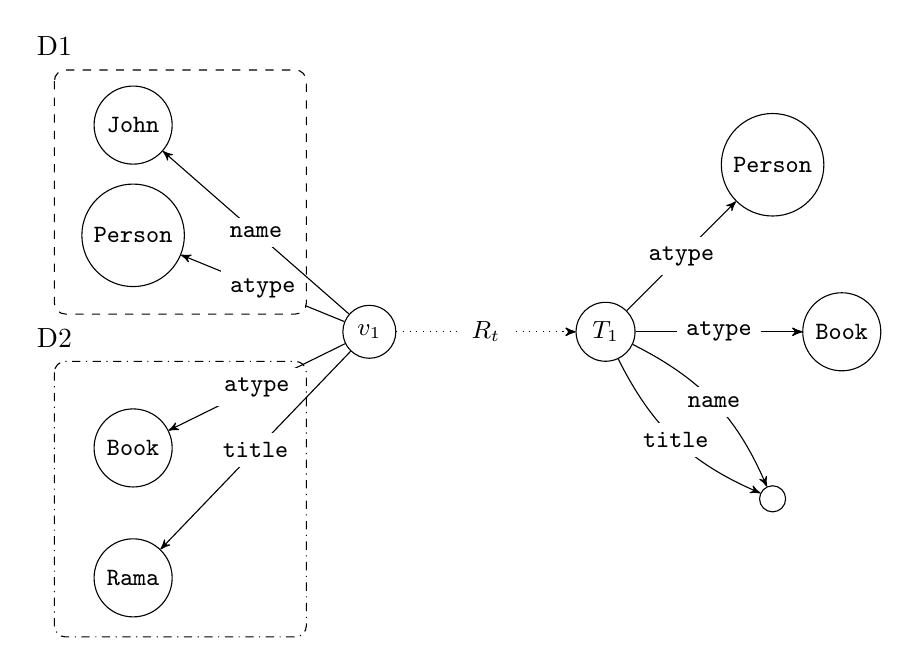
\begin{tikzpicture}[->,>=stealth',node distance=3cm,main node/.style={draw,circle,font=\small\ttfamily}]
\node (n1a) {};
\node[below of = n1a,yshift=-1cm] (n1b) {};

\node[main node,below of = n1a,yshift=1.125cm] (n1) {$v_1$};

\node[main node,left of = n1a,yshift=-.65cm] (person) {Person};
\node[main node,left of = n1b,yshift=.65cm] (doc) {Book};
\node[main node,left of = n1a,yshift=.75cm] (john) {John};
\node[main node,left of = n1b,yshift=-1cm] (rama) {Rama};

\coordinate (d1x) at ($ (person) + (-1,2.1) $);
\coordinate (d1y) at ($ (person) + (2.2,-1) $);
\draw[rounded corners,dashed]  (d1x) node[yshift=.3cm] {D1} rectangle (d1y);

\coordinate (d2x) at ($ (doc) + (-1,1.1) $);
\coordinate (d2y) at ($ (doc) + (2.2,-2.4) $);
\draw[rounded corners,dashdotted]  (d2x) node[yshift=.3cm] {D2} rectangle (d2y);

\node[main node,right of = n1] (t1) {$T_1$};
\node[main node,above right of = t1] (tperson) {Person};
\node[main node,right of = t1] (tdoc) {Book};
\node[main node,below right of = t1] (tvn) {$\varnothing$};

\path[every node/.style={fill=white,font=\small\ttfamily}]
(n1) edge node {\glssymbol{atype}} (person)
		edge node {name} (john)
		edge[dotted] node {$R_t$} (t1)
 edge node {\glssymbol{atype}} (doc)
		edge node {title} (rama)
		edge[dotted] node {$R_t$} (t1)
(t1) edge node {\glssymbol{atype}} (tperson)
		edge node {\glssymbol{atype}} (tdoc)
		edge node {\glssymbol{atype}} (tdoc)
		edge[bend left = 20] node {name} (tvn)
		edge[bend right = 20] node {title} (tvn)
;
\end{tikzpicture}